\documentclass[a4paper, 12pt]{report}
\usepackage[utf8]{inputenc}
\usepackage[swedish]{babel}
\usepackage{relsize}
\usepackage[backend=biber, style=alphabetic, sorting=ynt]{biblatex}
\usepackage{csquotes}
\usepackage{graphicx}
\usepackage{titlesec}
\usepackage{titling}
\usepackage{pgf-pie}
\usepackage{hyperref}

\emergencystretch=1em

\setcounter{secnumdepth}{0}

\bibliography{bibliography.bib}
\addbibresource{biliography.bib}

\author{Eddie Englund}
\title{Linux vs Windows\\[0.2em]\smaller{}En djupgående analys på prestanda skillnader mellan Microsoft Windows och Gnu/Linux}

\renewcommand{\abstractname}{Abstract}
\renewcommand{\abstract}{Abstract}
\renewcommand*{\bibfont}{\small}


\begin{document}

\begin{titlepage}

    \maketitle

    \begin{center}

    
        
\includegraphics[width=0.15\textwidth]{nti}\par\vspace{1cm}

    {\scshape\LARGE NTI Gymnasiet Gärdet \par}
    \vspace{1cm}
    {\scshape\Large Examensarbete/Master Thesis, April 2020\par}
	\vspace{1.5cm}
    \textbf{
    Student: Eddie Englund, eddie.englund@elev.ga.ntig.se även eddie.englund@protonmail.com}
    \vspace{0.2cm}

    Handledare NTIG: Haris Kasumović, Haris.Kasumovic@ntig.se
    \vspace{0.1cm}

    Examinator NTIG: Haris Kasumović, Haris.Kasumovic@ntig.se
    
    \end{center}
\end{titlepage}


\section{Sammanfattning}\label{sum}

    \begin{abstract}

    \end{abstract}

\tableofcontents



\section{Inledning}


    I dagens samhälle så präglas operativ-systemens värld av två stora jättar. Apple och Microsoft eller mer exakt deras operativstystem; macOS och Microsoft Windows. Men det finns ett tredje operativsystem som faktisk är grunden på bl.a Android och Apples macOS men också deras andra operativsystem IOS och det system kallas för Linux.


\section{Bakrund}

    Linux i sig självt är inte ett operativsystem. Däremot, så är Linux det som kallas för en ``kernel''\cite{redhat}. Det är det som är hjärtat eller kanshe lite bättre jämfört med hjärnan av operativsystemet. Kerneln är en typ av mellanhand, mellan mjukvaran och hårdvaran. Den hanterar minnen och processer men även också en del andra saker.

    Men eftersom att Linux är en kernel så finns det många så kallade distributioner utav det och dom är mer eller mindre operativsystem men med Linux som kärna. Den distributionen som jag har valt att använda är Manjaro\cite{manjaro}. Manjaro är en så kallad \textit{Arch based distro}. Den är baserad på en annan distro som heter Arch Linux som offta blir kallat för den bästa distron. Men, Manjaro gör det lättare att komma igång med och har dem flästa fördelarna med Arch.

    Men den största skillnaden mellan Gnu/Linux och Windows är att det inte är proprietär och har öppen källkod vilket betyder att vem som helst kan bidra med kod för att; göra kerneln eller distrobutionen bättre och lägga till fler användbara funktioner, men också att fixa buggar. Öppen källkod har även en annan fördel och det är att koden offtast inte är så kallad \textit{``bloated''}, alltså att det finns kod eller funktioner som inte behövs eller att kod kvaliten inte är bra. Detta leder till att prestandan på Linux är mycket hög. 
    
    Därför så vill jag ta reda på om prestandan mellan Linux (manjaro) och Microsoft Windows 10 har en uppenbar skillnad och om dom har det, varför? Jag vill dessutom veta vad konsensusen är inom utväcklar miljöer.

\subsection{Vad tror utväcklare?}

    För att ta reda på vad andra utväcklare har för hypotes/teori om prestandan mellan Liunux i allmänhet och Windows 10, varför prestandan skulle vara annorlunda, vilket operativstystem dom föredrar och varför.  Så delades det runt ett formulär runt om kring olika programerings/utväcklings forum men även genom kontakter lyckats skicka vidare formuläret i proffesionella utväcklingsmiljöer.

    Notera att formuläret var skrivet på Engelska för att kunna nå ut till så många utväcklare så möjligt.


    \vspace{8.7cm}


    \large {Which operating system would have superior performance in tasks like, compiling code, executing code or even intensive workloads like working in a program  like blender or unity?}

    \vspace{.2cm}

    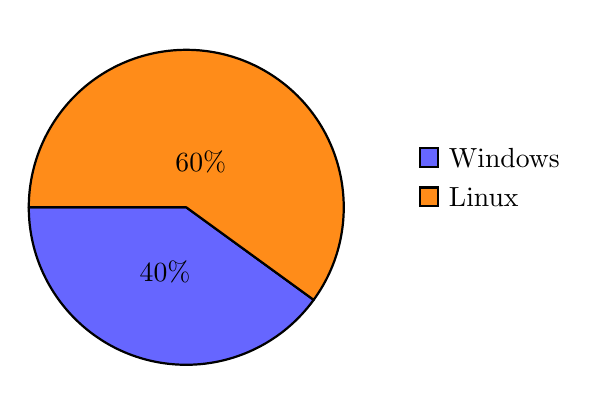
\begin{tikzpicture}
        \pie [rotate = 180, color = {blue!60, orange!90}, radius = 2, text = legend]
    {40/Windows,
     60/Linux}

    \end{tikzpicture}

    \cite{form}
    \vspace{1cm}

    \large {Which operating system would have superior performance in tasks like, compiling code, executing code or even intensive workloads like working in a program  like blender or unity?}

    \vspace{.5cm}


    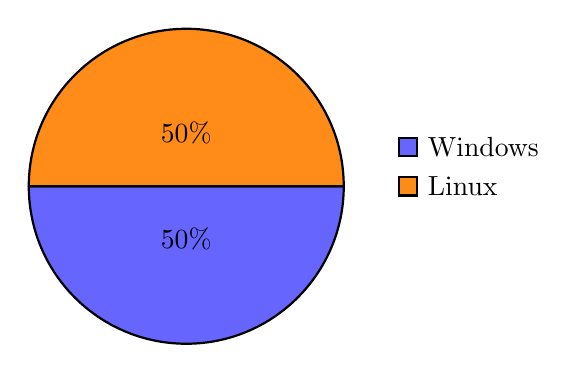
\begin{tikzpicture}
        \pie [rotate = 180, color = {blue!60, orange!90}, radius = 2, text=legend]
    {50/Windows,
     50/Linux}

    \end{tikzpicture}

    \cite{form}

    \vspace{1cm}


    \small{OBS! Det fanns några frågor som var alternativa, till exempel: att motivera sina svar.
    
    Vill ni läsa dessa motiveringar så finns dom här:} \smaller{\url{https://tinyurl.com/rccw2af}}


\section{Metod}



\section{Resultat}

\section{Analys/diskussion}



\section{Slutsats}


\printbibliography


\end{document}